To write specifications for protocols' rich semantics, I employed ``interaction
tree'' (ITree), a generic data structure for representing interactive programs
in the Coq programming language, introduced by \citet{itree}.  ITrees allow
specifying protocols as monadic programs that model valid implementations'
possible behavior.  The ITree specification can be interpreted into a tester
program, as discussed in later sections.

\subsection{Language definition}
\label{sec:itree-lang}
Consider an echo program, which keeps reading some data and writing it out
verbatim, until reaching EOF.  We can represent the program in Coq, with a
reference in C as:
\begin{multicols}{2}
\begin{coq}
  CoFixpoint echo :=
    c <- getchar;;
    if c is EOF
    then EXIT
    else
      putchar c;;
      echo.
\end{coq}
\columnbreak
\begin{cpp}
  void echo() {
    const char c = getchar();
    if (c == EOF)
      return;
    else {
      putchar(c);
      echo();
    }
\end{cpp}
\end{multicols}
Here the behavior after \ilc{getchar} depends on the value actually read.  The
monadic computation in Coq can be desugared into:
\begin{coq}
  CoFixpoint echo :=
    Bind getchar
         (fun c => if c is EOF
                 then EXIT
                 else Bind (putchar c)
                           (fun _ => echo)
         ).
\end{coq}
Such continuation-passing style can be represented as a tree of interactions.
To help readers better understand the interaction tree language, I first provide
a modified version of it that better shows its tree structure, and then explain
the actual type definition used in practice.

\begin{figure}
\begin{coq}
  CoInductive itreeM (E: Type -> Type) (R: Type) :=
    Ret     : R   -> itreeM E R
  | Trigger : E R -> itreeM E R
  | Bind    : forall {X : Type}, itreeM E X -> (X -> itreeM E R) -> itreeM E R.
\end{coq}
\caption{Mock definition of interaction trees.}
\label{fig:mock-itree}
\end{figure}

\begin{figure}
  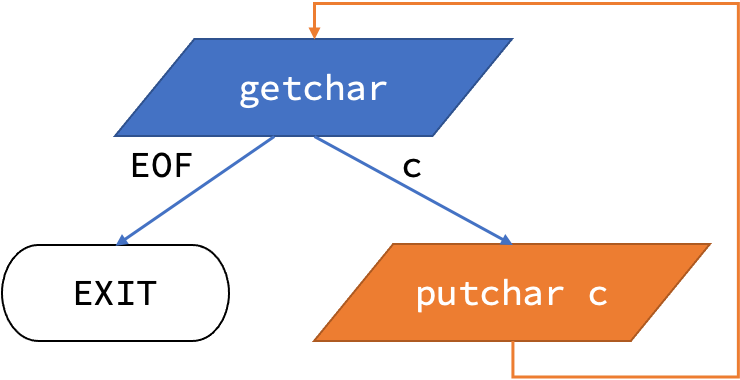
\includegraphics[width=.5\linewidth]{figures/echo-itree}
  \caption{Interaction tree for echo program}
  \label{fig:echo-itree}
\end{figure}

\paragraph{Mock interaction trees}
As shown in \autoref{fig:mock-itree}, a mock interaction tree (\ilc{itreeM}) has
two kinds of leaves, \ilc{Ret} and \ilc{Trigger}, and has internal nodes
constructed by \ilc{Bind}:
\begin{itemize}
\item \ilc{(Ret r)} represents a pure computation that yields a value \ilc r.
  In the echo example, \ilc{EXIT} halts the program with return value zero:
\begin{coq}
  Definition EXIT := Ret 0.
\end{coq}

\item \ilc{(Trigger e)} performs an impure event \ilc e and returns its result.
  Here \ilc{(e: E R)} is an event whose result is of type \ilc R.  For example,
  \ilc{getchar} has result type \ilc{char}, and \ilc{putchar}'s result type is
  \ilc{unit} (which corresponds to \inlinec{void} in C/C++, or \ilc{()} in
  Haskell).  These effective programs are constructed by triggering standard I/O
  events:
\begin{coq}
  Variant stdioE: Type -> Type := (* event type *)
    GetChar:         stdioE char
  | PutChar: char -> stdioE unit.
  
  Definition getchar           : itreeM stdioE char := Trigger  GetChar.
  Definition putchar (c: char) : itreeM stdioE unit := Trigger (PutChar c).
\end{coq}
\item \ilc{(Bind m k)} binds the return value of \ilc m to the continuation
  function \ilc k.  It first runs program \ilc m until it returns some value of
  type \ilc X.  The return value \ilc{(x: X)} then instantiates \ilc k into the
  following computation \ilc{(k x: itreeM E R)}.  This corresponds to the
  monadic \ilc{(;;)} syntax:
\begin{coq}
  Notation "x <- m1;; m2" := (Bind m1 (fun x => m2)).
  Notation "m1;; m2"      := (Bind m1 (fun _ => m2)).
\end{coq}

As illustrated in \autoref{fig:echo-itree}, each possible return value \ilc x is
an edge that leads to the child it instantiates, {\it i.e.}, \ilc{(k x)}.  In this
way, the \ilc{Ret} and \ilc{Trigger} nodes are connected into a tree
structure.
\end{itemize}

The mock interaction tree provides an intuitive continuation-passing structure
for representing impure programs.  However, to implement dualization
effectively, we need to revise the language definition of monadic binding.

\paragraph{Practical interaction trees}

\begin{figure}
\begin{coq}
  CoInductive itree (E: Type -> Type) (R: Type) :=
    Pure   : R -> itree E R
  | Impure : forall {X : Type}, E X -> (X -> itree E R) -> itree E R.
\end{coq}
\caption{Formal definition of interaction trees (simplified)}
\label{fig:itrees}
\end{figure}

Instead of binding a program to a continuation, ITree binds a single impure
event, as shown in \autoref{fig:itrees}.  I use \ilc{(Impure e k)} to
replace \ilc{(Bind (Trigger e) k)} representations in \ilc{itreeM}.
A \ilc{Pure} computation cannot be bound to a continuation, and must be the leaf
of an ITree.\footnote{For readability, the ``practical'' ITree definition is a
simplified version from \citet{itree}.  Here \ilc{Pure} and \ilc{Impure}
correspond to the \ilc{Ret} and \ilc{Vis} constructors.  I dropped the \ilc{(Tau
: itree E R -> itree E R)} constructor, which carries no semantics and is used
for satisfying Coq's guardedness condition.}

The \ilc{Ret}, \ilc{Trigger}, and \ilc{Bind} constructors introduced in
\ilc{itreeM} have equivalent representations in \ilc{itree}, so we can still
write programs in the monadic syntax:
\begin{coq}
  Definition ret {E R} : R -> itree E R := Pure.
  
  Definition trigger {E R} (e: E R) : itree E R := Impure e Pure.

  CoFixpoint bind {X E R} (m: itree E X) (f: X -> itree E R) : itree E R :=
    match m with
    | Pure   x   => f x
    | Impure e k => Impure e (fun r => bind (k r) f)
    end.

  Notation "x <- m1;; m2" := (bind m1 (fun x => m2)).
  Notation "m1;; m2"      := (bind m1 (fun _ => m2)).

  CoFixpoint translateM {E R} (m: itreeM E R) : itree E R :=
    match m with
    | Ret     r => ret r
    | Trigger e => trigger e
    | Bind m1 k => x <- translateM m1;; translateM (k x)
    end.
\end{coq}

\subsection{QAC in ITrees}
\label{sec:qac-itree}
The ITree specification language is a superset of the QAC language family.  Any
nondeterministic server model in \autoref{def:server} can be translated into an
interaction tree that receives requests of type $Q$, sends responses of type
$A$, and makes internal choices of type $C$.  The ITree's event type is defined
as follows:
\begin{coq}
  Variant qaE: Type -> Type :=
    Recv: qaE Q           (* receive a request *)
  | Send: A -> qaE unit.  (* send a response   *)

  Variant choiceE: Type -> Type :=
    Choice: choiceE C.    (* make an internal choice *)

  Definition qacE: Type -> Type := qaE +' choiceE.
\end{coq}
Here \ilc{qacE} is a sum type of \ilc{qaE} and \ilc{choiceE} events, meaning
that the server's events are either sending/receiving messages or making
internal choices.  I split the event types because they'll be handled
differently when I derive the tester later in this chapter.

Now we can define the interaction tree of a nondeterministic server with loop
body \ilc{sstep} and initial state \ilc s:
\begin{coq}
  CoFixpoint server (sstep: Q -> C -> sigma -> A * sigma) (s: sigma) : itree qacE void :=
    c <- trigger Choice;;
    q <- trigger Recv;;
    let (a, s') := sstep q c s in
    trigger (Send a);;
    server sstep s'.
\end{coq}
The \ilc{server} is a recursive program that iterates over state \ilc{(s:
sigma)}.  In each iteration, it makes an internal choice \ilc{(c: C)} and
receives a request \ilc{(q: Q)}.  It then computes the response \ilc{(a: A)} and
the post state \ilc{(s': sigma)} using the \ilc{sstep} state monad function,
sends back the response, and recurses with the post state.

The rest of this chapter shows how to derive interactive tester programs from
specifications written as ITrees.
